\section{Überblick über den Aufbau und Datenfluss}

\begin{figure}[htbp]
\centering
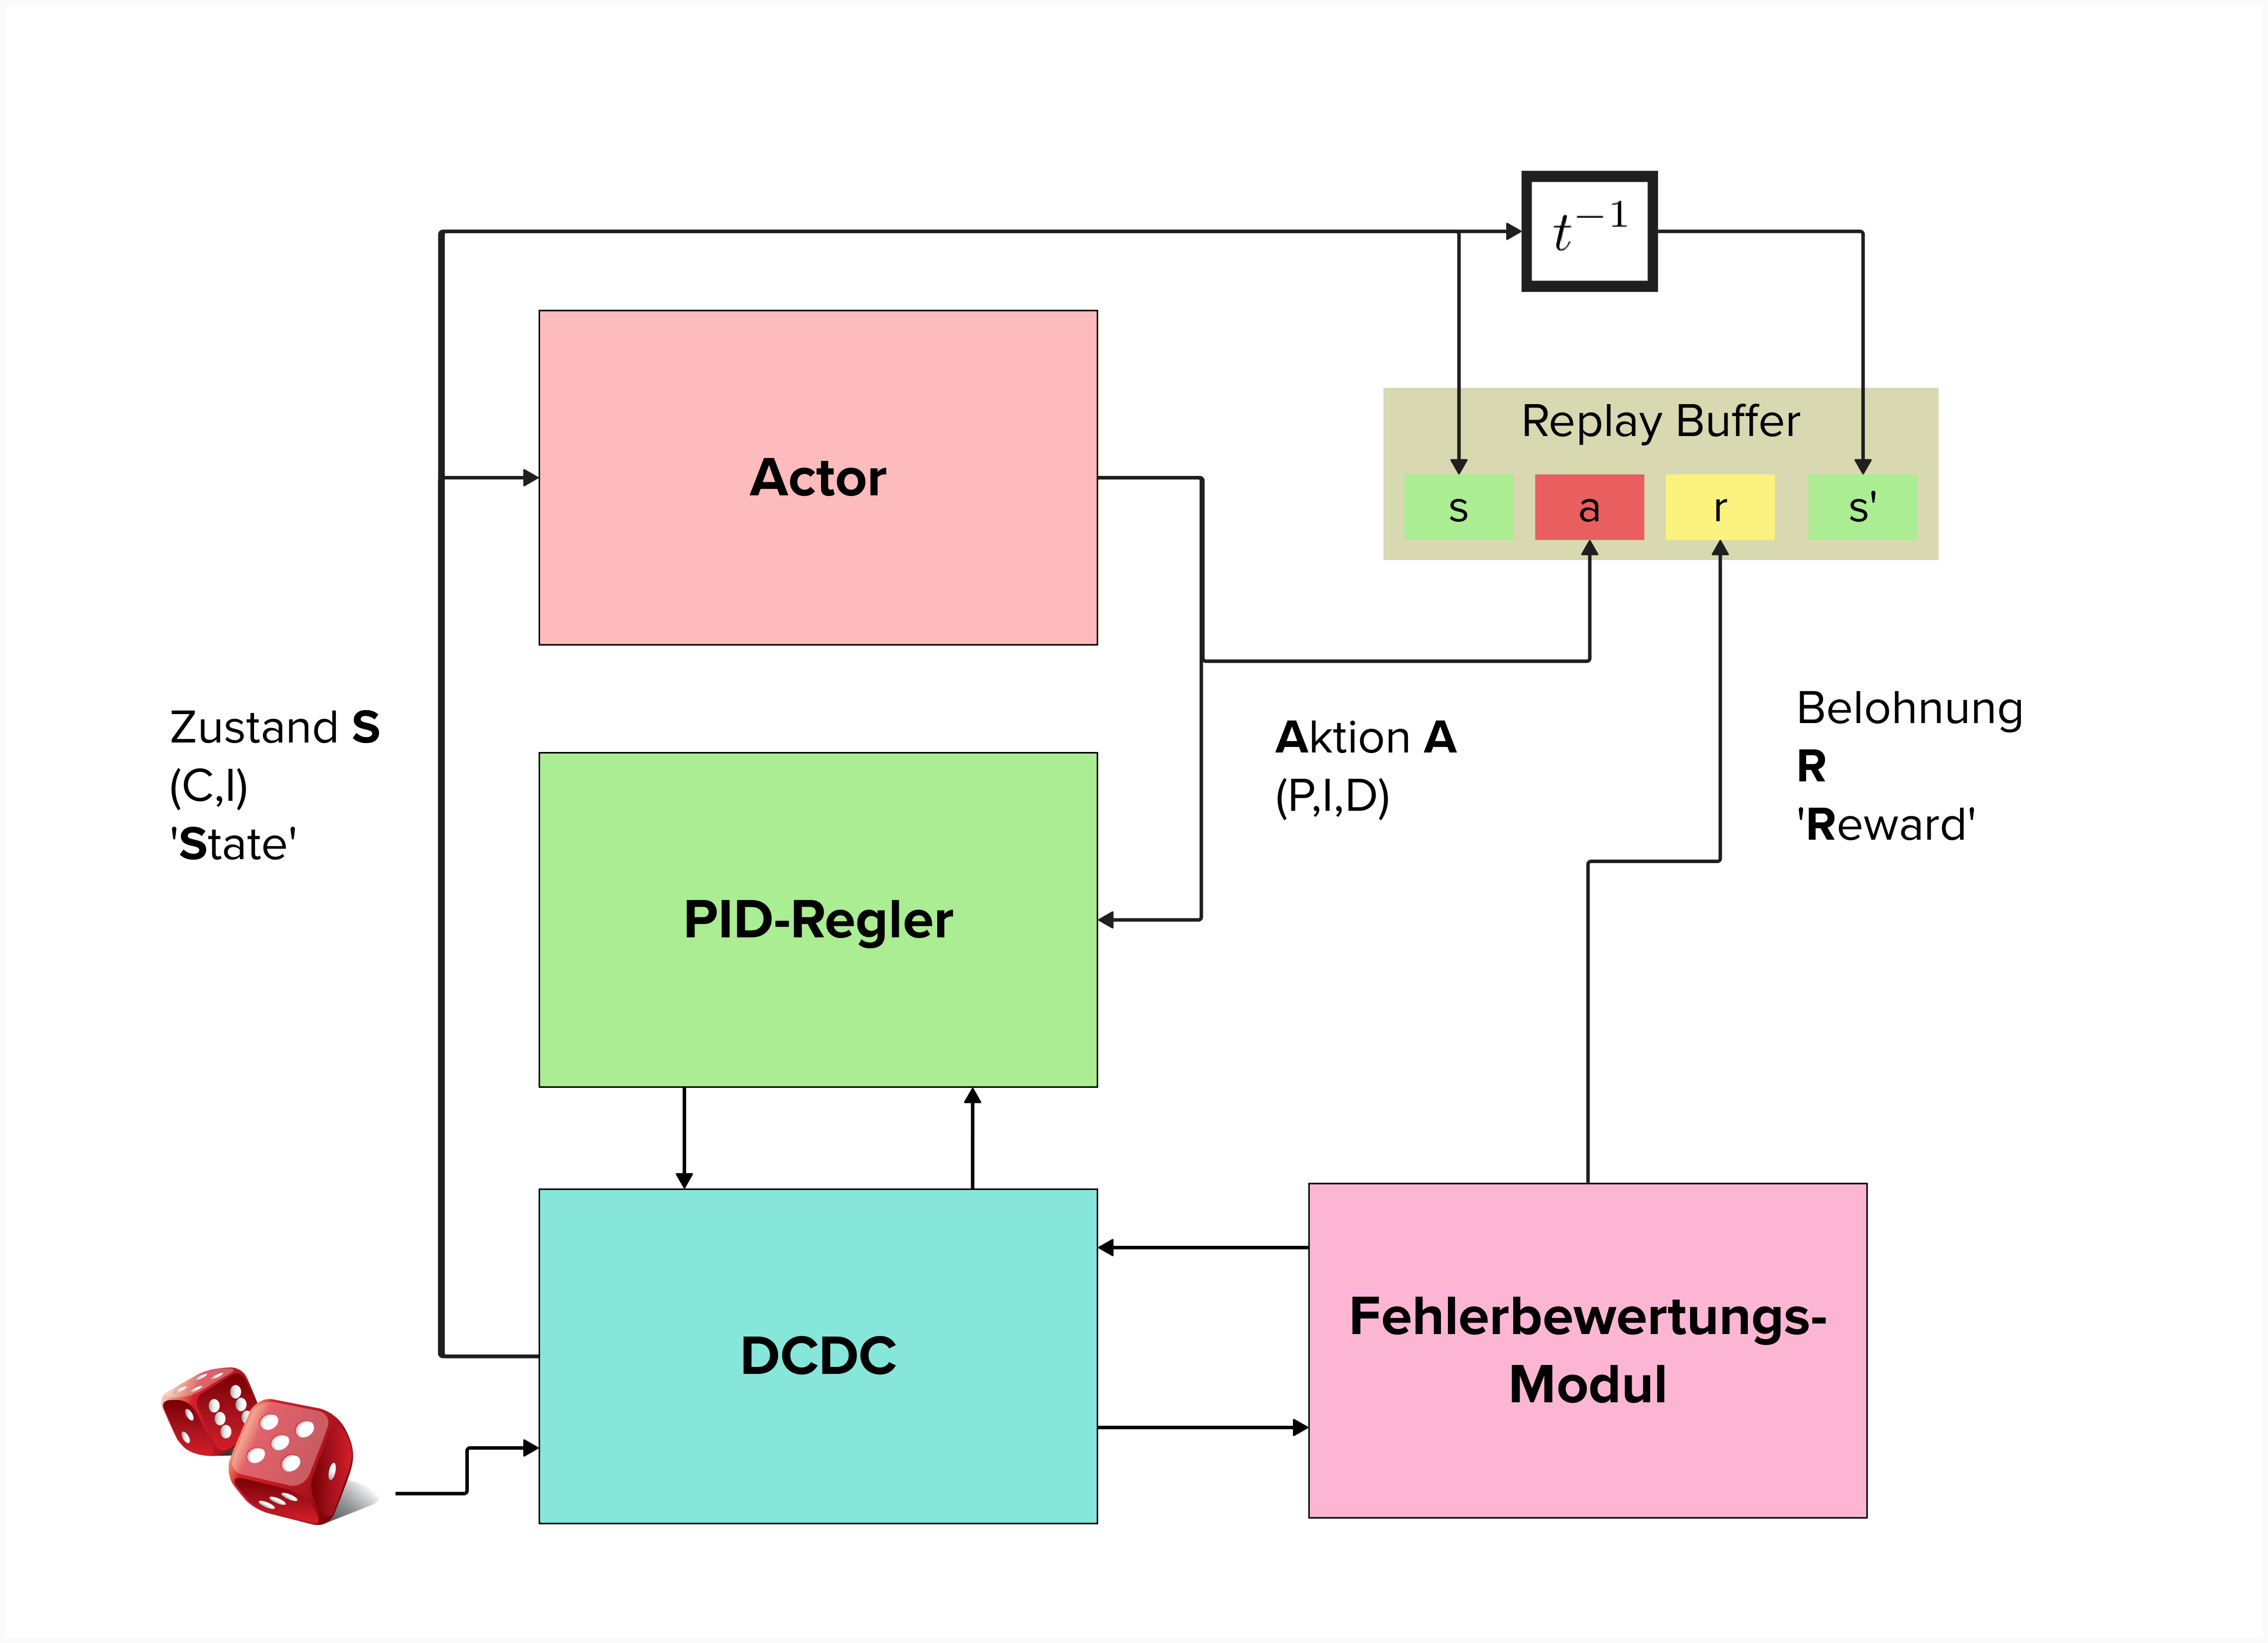
\includegraphics[width=0.72\textwidth]{3Experiment/2Experiment/0Experiment_Grob.png}
\caption{Detaillierte Darstellung des Systems zur Datensammlung für das Training des neuronalen Netzes.}
\label{fig:data_collection_system}
\end{figure}


\paragraph{Einleitung}
Dieser Abschnitt gewährt einen Überblick über die Struktur und den Datenfluss innerhalb Modueln\ref{fig:data_collection_system} Die detaillierten theoretischen Grundlagen der Systemkomponenten wurden im Grundlagenteil dieser Arbeit ausführlich behandelt. An dieser Stelle werden die Funktionen und Interaktionen der einzelnen Module im Kontext der Datenerfassung für das Training des neuronalen Netzes dargestellt.


\paragraph{Datenfluss im Reinforcement Learning System}
Im Zentrum des Datenflusses unseres Systems steht die Befüllung des Replay Buffers \ref{fig:replay_buffer}\ref{sec:Replay Buffers} mit wertvollen Informationen für das Training des Agenten. Diese Informationen bestehen aus den Zuständen der Schaltung, den getroffenen Aktionen des Agenten und den daraus resultierenden Belohnungen. 


\subsection{Makrozyklus: Systemüberblick und Datenauswertung}
Im Makrozyklus unseres Systems, wie in der beigefügten Abbildung \ref{fig:makrozyklus} dargestellt, konzentrieren wir uns auf die Simulation der Systemzustände und die anschließende Datenauswertung für das Training des neuronalen Netzwerks. Dieser Zyklus beinhaltet die Sammlung von Daten über verschiedene Zustände der Schaltung, einschließlich der Simulation der Systembedingungen sowie der Auswertung und Trainierung des neuronalen Netzwerks. Jeder Schritt in diesem Zyklus trägt dazu bei, ein umfassendes Verständnis der Systemdynamik zu entwickeln, was für die effiziente Anpassung des Netzwerks entscheidend ist. Der Makrozyklus wurde hauptsächlich in Python implementiert, um die Flexibilität und Erweiterbarkeit der Datenverarbeitungs- und Analyseprozesse zu maximieren.

\subsection{Mikrozyklus: Detailanalyse und Regelungsstrategien}

Im Mikrozyklus liegt der Fokus auf der Simulation der Verhaltensweisen des DC-DC-Konverters unter verschiedenen Bedingungen, insbesondere im Zusammenspiel mit einem PID-geregelten System. Diese Detailanalyse ermöglicht es, fein abgestimmte Regelungsstrategien zu entwickeln, die eine präzise Steuerung der Systemkomponenten unter variierenden Betriebsbedingungen erlauben. Der Mikrozyklus wurde in SystemC implementiert, was sich als besonders effizient für die Transientenanalyse einzelner Komponenten und die Simulation unter unterschiedlichen Bedingungen erwiesen hat. Die Durchführung eines Mikrozyklus auf einer Standard-CPU dauert etwa 0,3 Sekunden, was die schnelle Reaktionsfähigkeit und Anpassungsfähigkeit unseres Systems unterstreicht.

\begin{figure}[htbp]
\centering
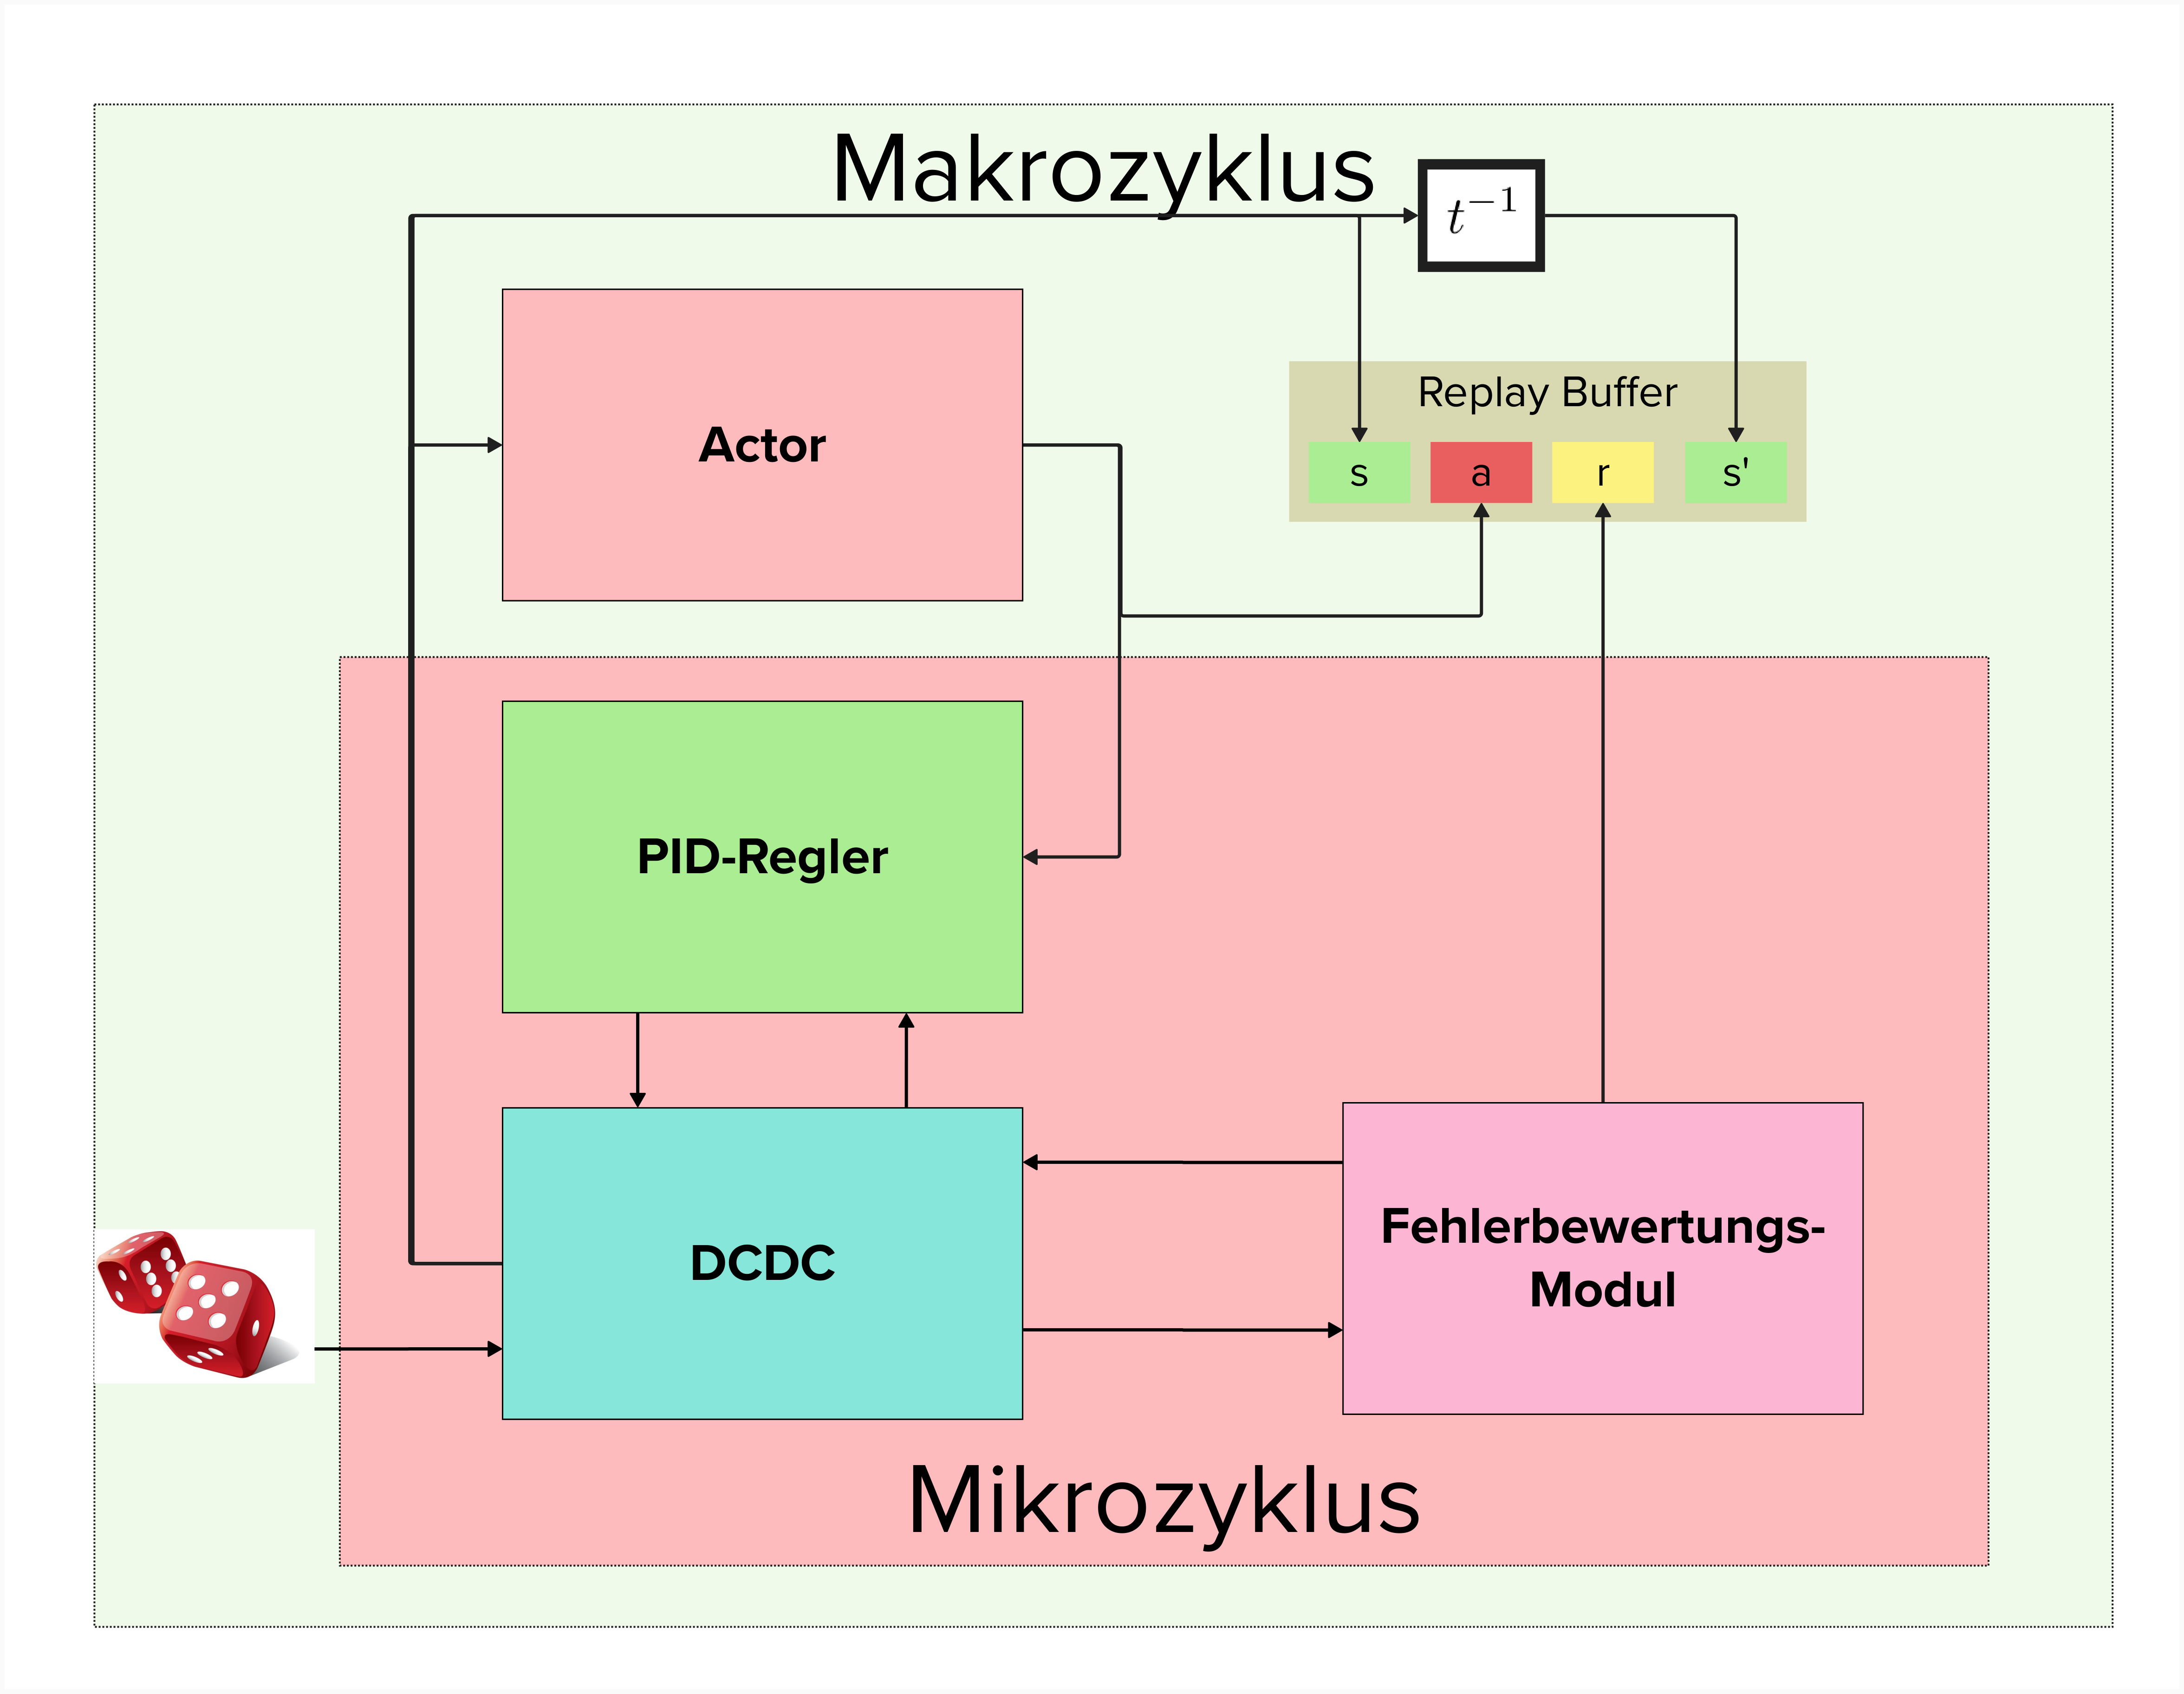
\includegraphics[width=0.8\textwidth]{3Experiment/2Experiment/0Zeitliche_Dimensio.png}
\caption{Visualisierung des Mikro- und Makrozyklus mit Darstellung der zeitlichen Unterteilung in zwei Dimensionen.}
\label{fig:makrozyklus}
\end{figure}




\begin{figure}[htbp]
\centering
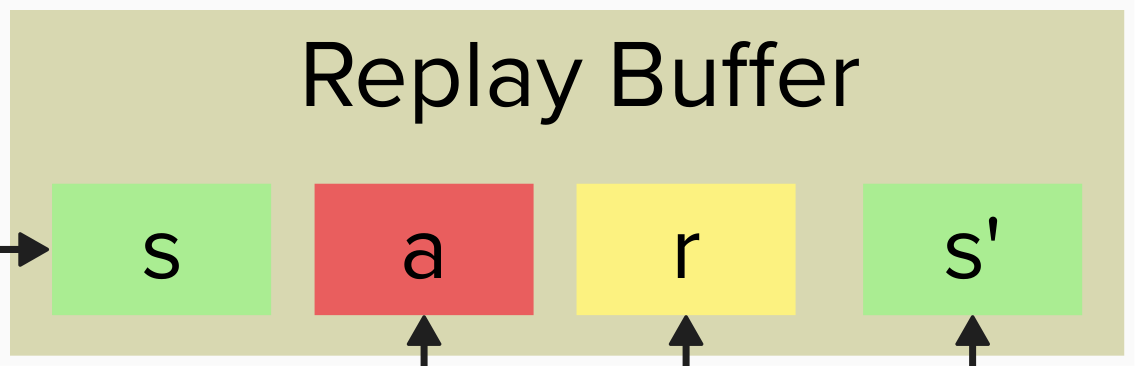
\includegraphics[width=0.4\textwidth]{3Experiment/2Experiment/0Replay_Buffer_short.png}
\caption{Schematische Darstellung des Replay Buffers, der als Datenspeicher für das Reinforcement Learning System dient. Er zeichnet die Sequenz der erlebten Zustände \( s \), Aktionen \( a \), Belohnungen \( r \) und nachfolgenden Zustände \( s' \) auf, welche für die stetige Anpassung und Verbesserung des Agenten verwendet werden.}
\label{fig:replay_buffer}
\end{figure}

\subsection{ Makrozyklus Schritt 1: Zustandssimulation und Datengenerierung}

Die Generierung der Schaltungszustände, die als Input für den Lernprozess dienen, erfolgt mittels einer Zufallsfunktion. In der realen Welt erfolgen Zustandsübergänge in einer physischen Schaltung in langen Zeitintervallen, was eine direkte Simulation unpraktisch macht. Deshalb greifen wir auf eine alternative Methode zurück:

\begin{itemize}
    \item Initial wird über eine Gleichverteilung ein Degenerationszustand der Schaltung simuliert. Die zufällige Auswahl dieser Zustände geschieht innerhalb festgelegter Grenzen, um eine Vielfalt an möglichen Zuständen zu gewährleisten.
	\item Der simulierte Zustand wird durch einen Satz von Kapazitäts- und Induktivitätswerten dargestellt. Diese Werte werden durch den "Würfel" im System visualisiert \ref{fig:state_generation}, wobei die Pfeile vom Würfel zu den Zustandsvariablen C und L diesen Prozess der zufälligen Zustandsgenerierung abbilden.
\end{itemize}

In diesem Projekt werden exemplarische Einstellungen für die Zustandsgenerierung verwendet, die eine Annäherung an realitätsnahe Bedingungen darstellen. Bei einer Überführung in praktische Anwendungen würden diese Einstellungen so angepasst, dass sie mit den in der Realität verifizierten Werten übereinstimmen. Die aktuellen Grenzwerte für die Zustandsgenerierung sind wie folgt definiert:

\begin{itemize}
    \item Untergrenze: \( \text{Induktivität} = 5.0 \times 10^{-4} \), \( \text{Kapazität} = 1.0 \times 10^{-6} \)
    \item Obergrenze: \( \text{Induktivität} = 5.0 \times 10^{-2} \), \( \text{Kapazität} = 1.0 \times 10^{-4} \)
\end{itemize}

\begin{figure}[htbp]
\centering
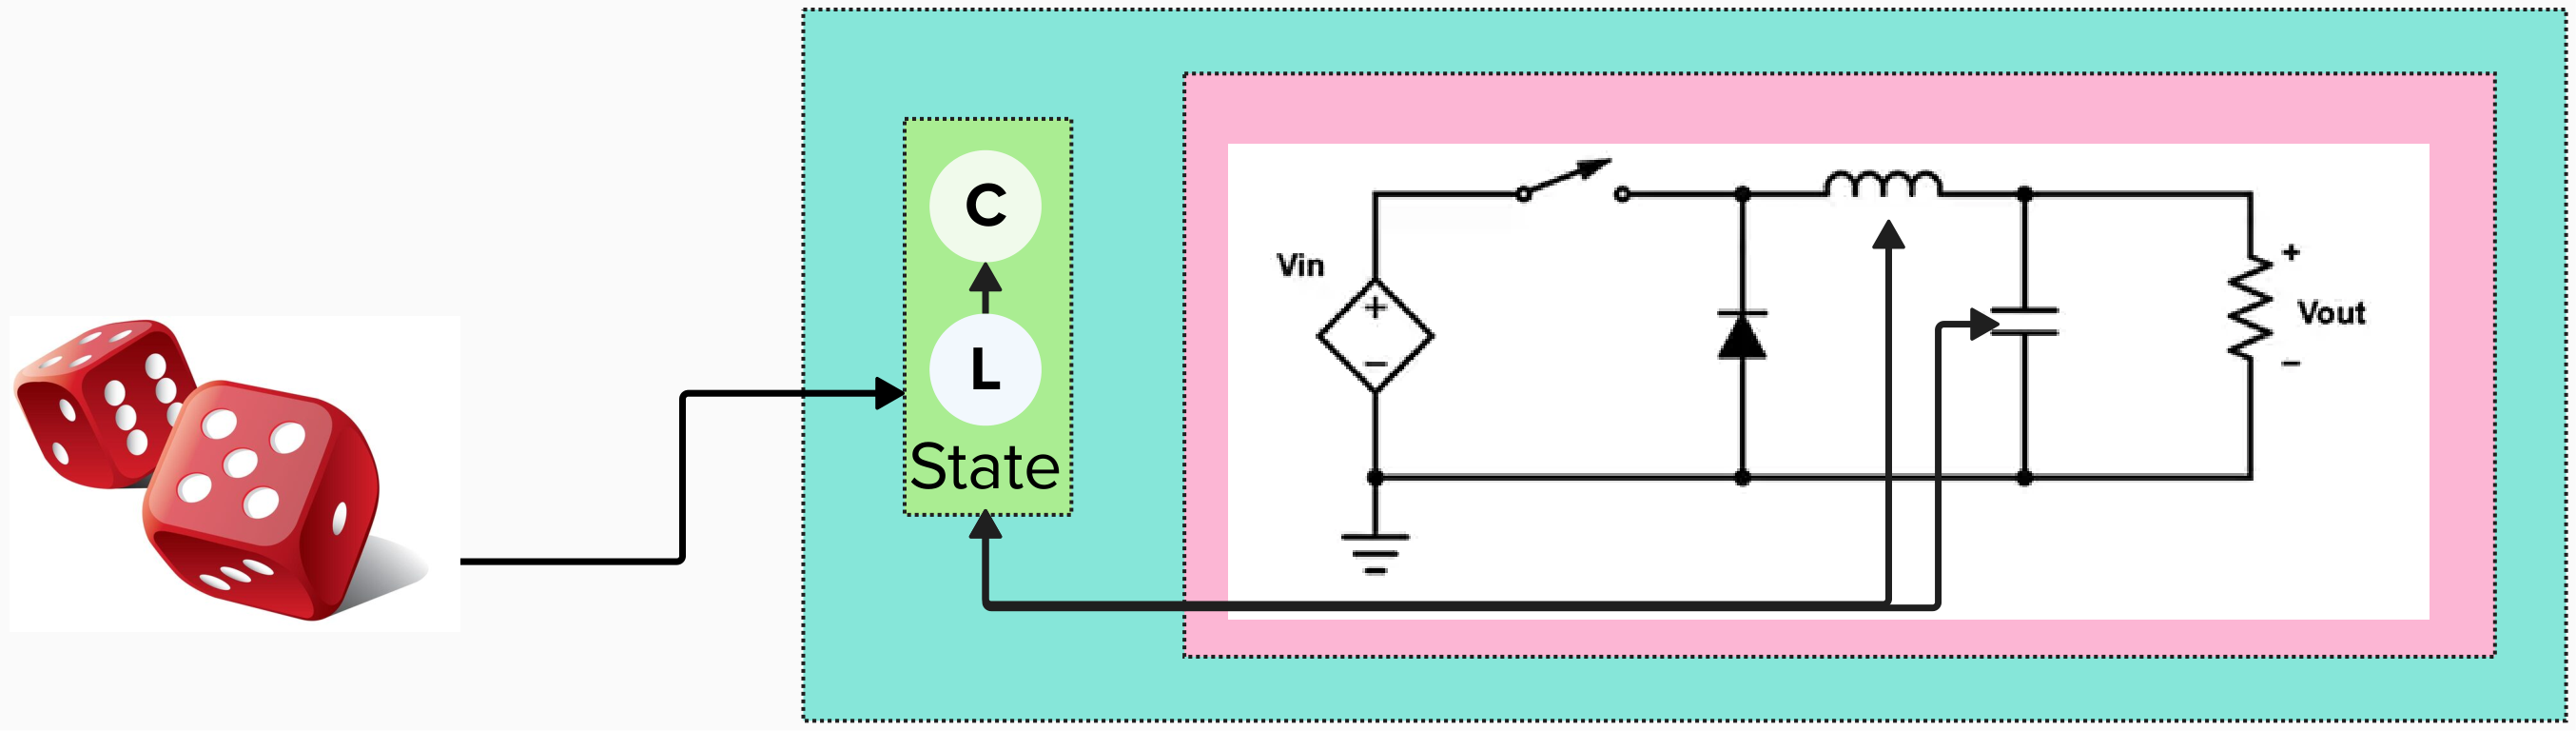
\includegraphics[width=0.7\textwidth]{3Experiment/2Experiment/1Random_Set_State.png}
\caption{Visualisierung der Zustandsgenerierung mit dem Würfel und die Setzung der Werte in der DCDC-Schaltung.}
\label{fig:state_generation}
\end{figure}

\subsection{Makrozyklus Schritt 2: Entscheidungsfindung durch den Actor}

Nachdem der initiale Schaltungszustand durch eine Zufallsverteilung generiert wurde, kommt der Actor ins Spiel, der auf Basis der aktuellen Kapazitäts- (C) und Induktivitätswerte (L) Entscheidungen trifft. Der Actor, ein wesentlicher Bestandteil des Reinforcement Learning Systems, ist eine komplexe Funktion, die sich aus mehreren Gewichtungen (weights) und Verzerrungen (biases) zusammensetzt. Diese werden im Laufe des Vorwärtsdurchlaufs (Forward Propagation \ref{sec: Forward Propagation}) durch das Netzwerk multipliziert und summiert.

\begin{itemize}
		\item Innerhalb des Actors wird die Eingabe durch jede Schicht des neuronalen Netzwerks transformiert, wobei nach jedem Schichtdurchgang eine nicht-lineare Aktivierungsfunktion \ref{eq:activation_function} angewandt wird, um die Linearität der Operationen zu durchbrechen.
		\item Im spezifischen Kontext unseres Systems ist die Aktivierungsfunktion der letzten Schicht eine  Hyperbelfunktion (tanh), die die Ausgabe des Netzwerks beeinflusst und zu einem komplexen, nicht-linearen Ergebnis führt.
\end{itemize}

Die Ausgabe des Actors sind die PID-Werte, die für die Steuerung des nächsten Schrittes im System verwendet werden. Diese Werte sind das Resultat des durch die tanh-Funktion modifizierten Outputs und stellen somit eine fein abgestimmte Reaktion auf den Zustand der Schaltung dar. Diese Werte werden anschließend skaliert, um realistische PID-Reglerparameter zu erhalten:

\begin{itemize}
	\item Der Proportionalwert (Kp) wird zwischen 0 und 10 skaliert.
	\item Der Integralwert (Ki) wird zwischen 0 und 1 skaliert.
	\item Der Differentialwert (Kd) wird zwischen 0 und 0.1 skaliert.
\end{itemize}

Diese Skalierung ist entscheidend, um die Ausgangswerte des neuronalen Netzes in praktikable Steuerparameter zu überführen. Die Transformation gewährleistet, dass die PID-Werte in einem Bereich liegen, der für die Regelung des Systems adäquat ist und reflektiert die praktischen Anforderungen an die Systemsteuerung. 


\begin{figure}[htbp]
\centering
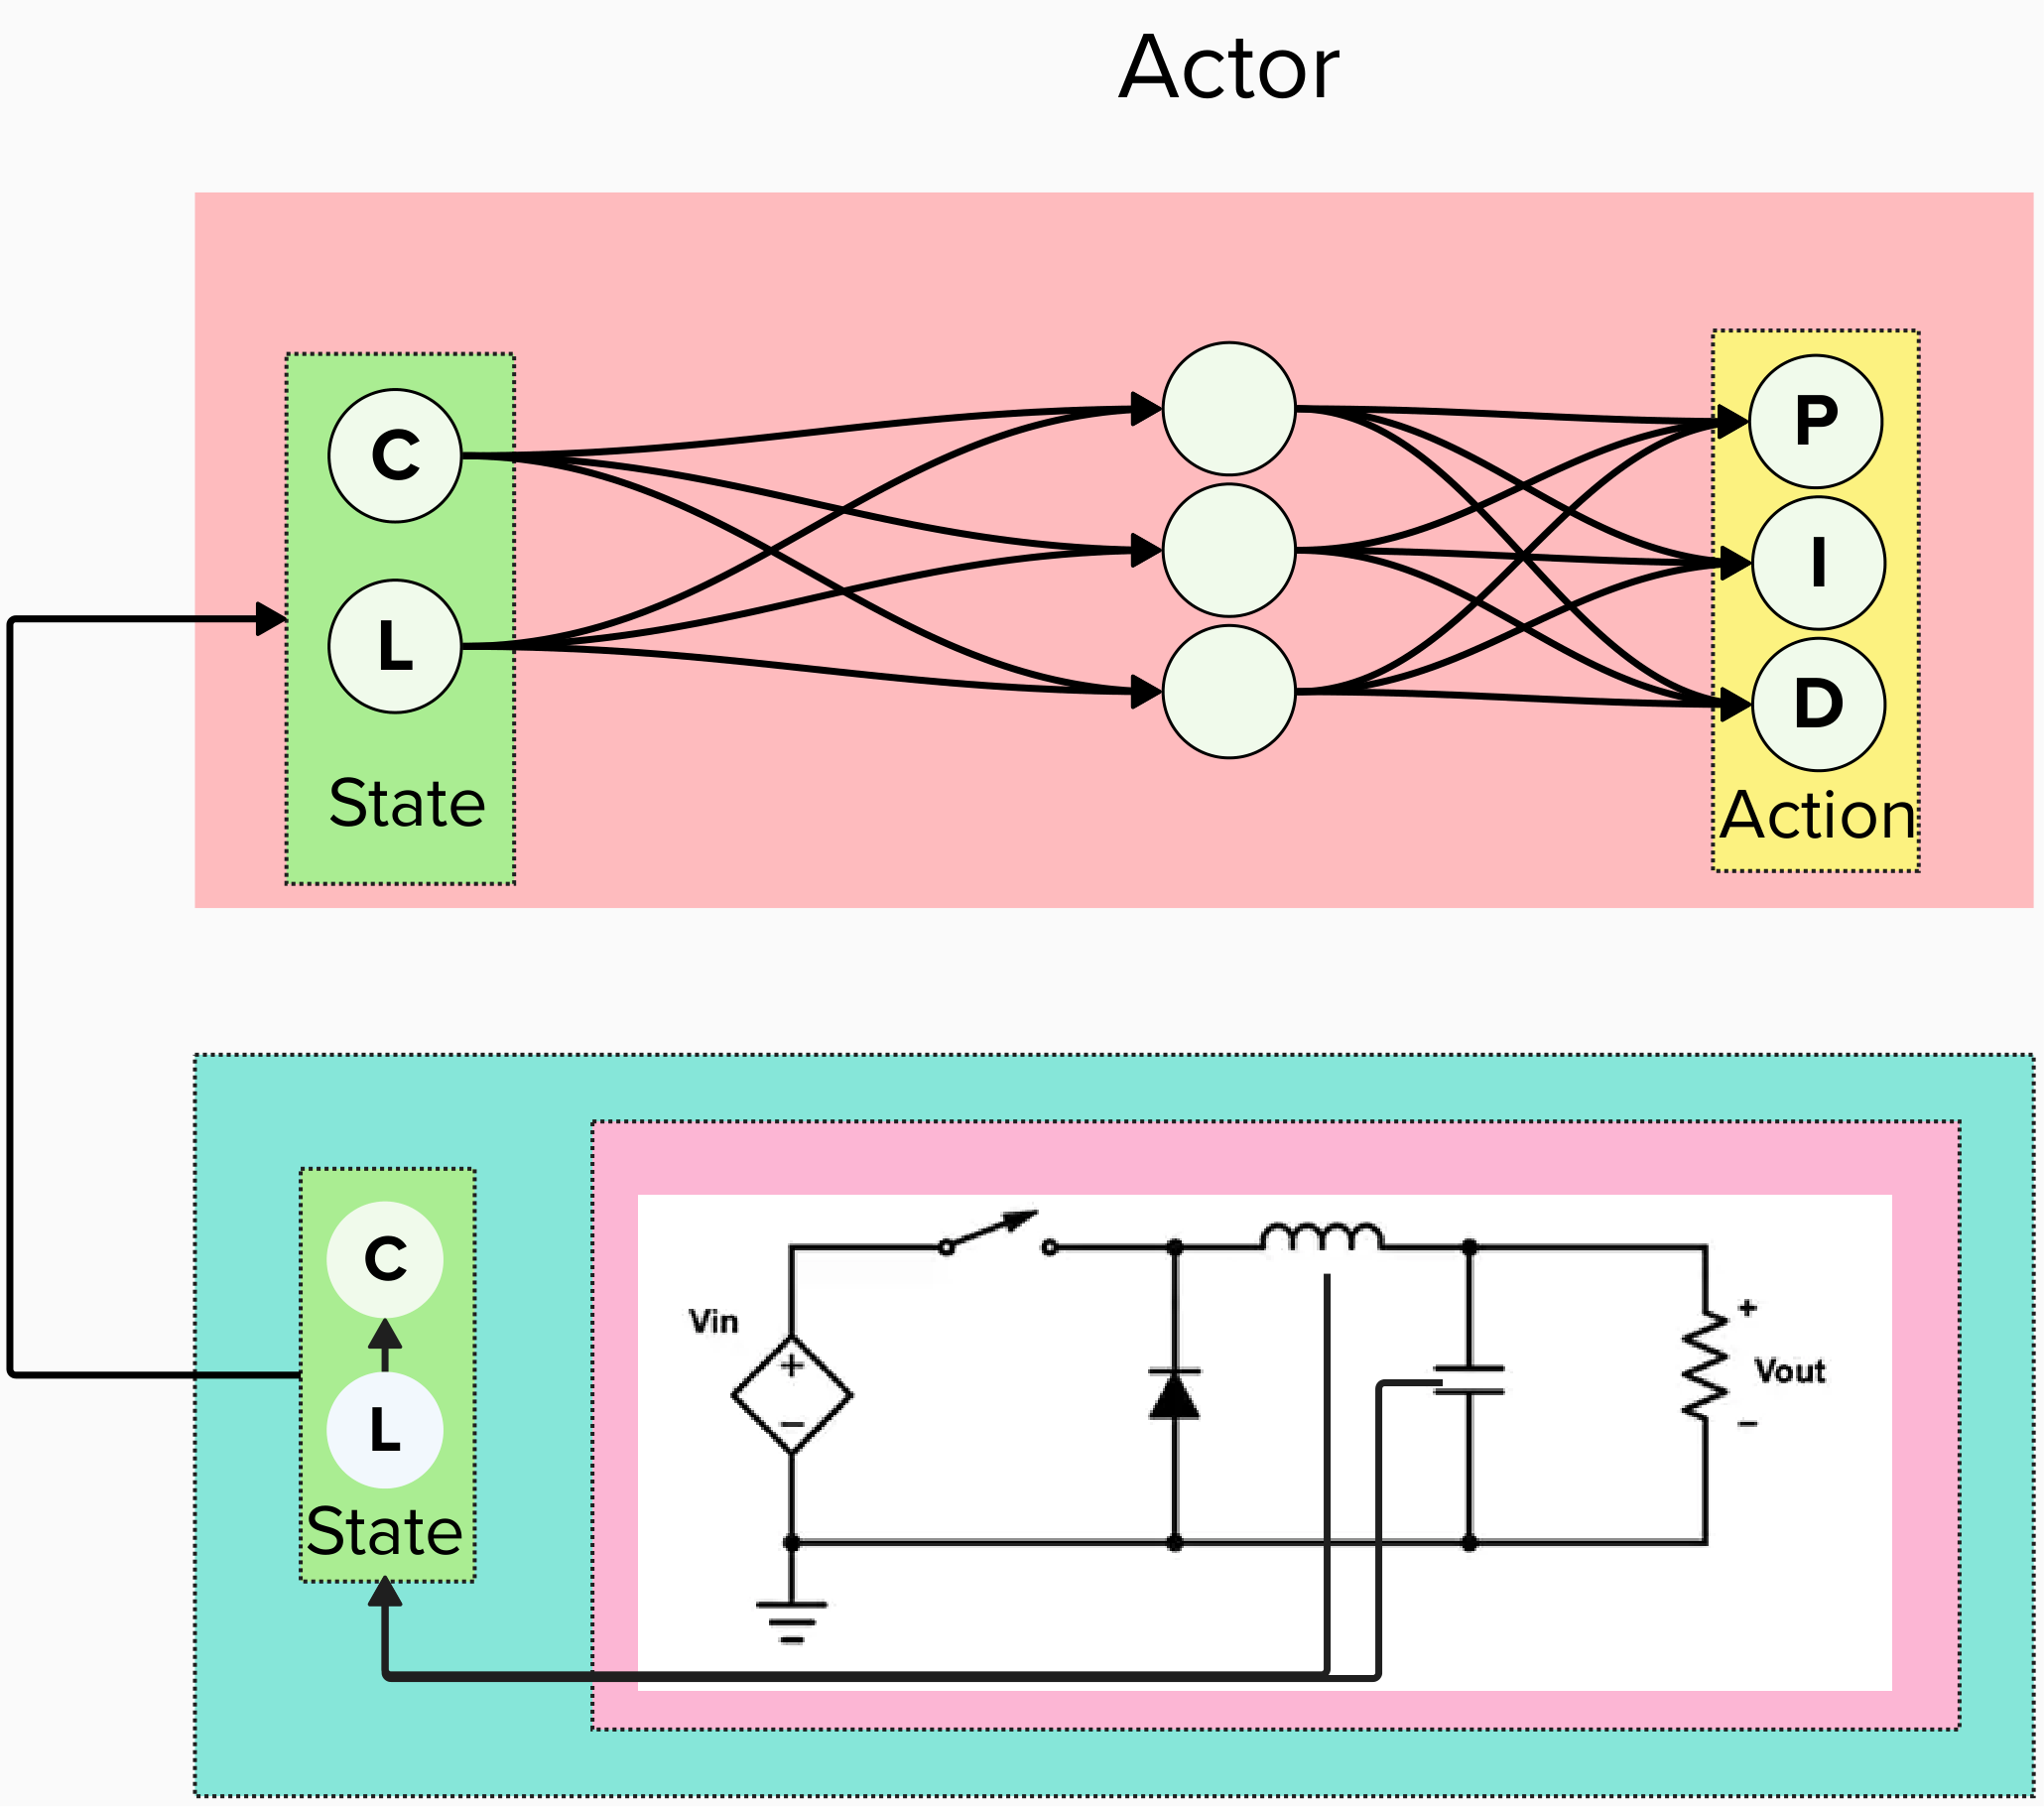
\includegraphics[width=0.5\textwidth]{3Experiment/2Experiment/2Actor.png}
\caption{Die Forward Propagation im Actor-Modul, die den Zustand S (C, L) aufnimmt und über ein mehrschichtiges neuronales Netzwerk PID-Aktionswerte ausgibt.}
\label{fig:actor_decision_making}
\end{figure}




\subsection{Gesamtdarstellung des Regelkreises mit PID-gesteuertem DCDC-Konverter}
\label{sec:Gesamtdarstellung_Regelkreis}

Dieser Abschnitt bietet einen umfassenden Überblick über den Regelkreis, der einen PID-Regler, einen Pulsweitenmodulator (PWM) und einen DCDC-Konverter umfasst. Im Mittelpunkt steht die Interaktion dieser Komponenten, die gemeinsam eine konstante Ausgangsspannung gewährleisten. Die Mikroebene der Simulation wird besonders hervorgehoben, um die Auswirkungen der Wechselwirkungen zwischen den einzelnen Elementen auf die Gesamtleistung des Systems zu verdeutlichen.
Abbildung \ref{fig:Regelkreis_Überblick} veranschaulicht den gesamten Regelkreis inklusive des PID-gesteuerten DCDC-Konverters.

\paragraph{Interaktion der Regelkreiskomponenten}
Der Regelungsprozess beginnt mit den vom Actor gelieferten PID-Koeffizienten \( K_p, K_i, \) und \( K_d \), die den PID-Regler ansteuern (siehe Abschnitt \ref{sec:PID-Regler}). Der Regler vergleicht kontinuierlich die aktuelle Spannung mit dem Referenzwert und generiert ein Signal zur Korrektur, das an den PWM weitergeleitet wird.

\paragraph{Funktionsweise des Pulsweitenmodulators (PWM)}
Der PWM-Modulator (Abschnitt \ref{sec:PWM_Grundlagen}) transformiert das Signal des PID-Reglers in eine pulsbreitenmodulierte Form, die den DCDC-Konverter ansteuert. Dieser Konverter sorgt für die Umwandlung der Eingangsspannung in eine stabile Ausgangsspannung. Die Signalverarbeitung im PWM bestimmt die Schaltfrequenz des Transistors im Konverter, um die Last angemessen zu versorgen.

\paragraph{Rolle des DCDC-Konverters}
Der DCDC-Konverter spielt eine zentrale Rolle im Regelkreis, indem er die Energie der Versorgungsspannung in eine nutzbare Ausgangsspannung umwandelt(siehe Abschnitt \ref{sec:DCDC_Konverter}) . Die Arbeitsweise des Konverters ist eng mit den PWM-Signalen verknüpft, welche das Öffnen und Schließen des Transistors steuern. Die PWM regelt die Impulsbreite basierend auf den Steuerbefehlen des PID-Reglers. Diese Impulse beeinflussen das Tastverhältnis und damit die Energiemenge, die durch den Transistor geleitet wird. Die Energie wird in der Induktivität gespeichert und als Strom an die Last abgegeben, wobei die Kapazität als Puffer dient. Änderungen in der Last führen zu Spannungsschwankungen, die der PID-Regler erfasst und ausgleicht, um eine stabile Ausgangsspannung zu gewährleisten.

\paragraph{Integration von Simulation und Realität}
Die Simulation des Regelkreises erfolgte in SystemC, wobei der PID-Regler direkt aus mathematischen Modellen abgeleitet und der PWM sowie der DCDC-Konverter für eine genauere Analyse implementiert wurden. Dies ermöglicht einen Ausgleich zwischen Genauigkeit und Simulationsgeschwindigkeit.


\begin{figure}[htbp]
    \centering
    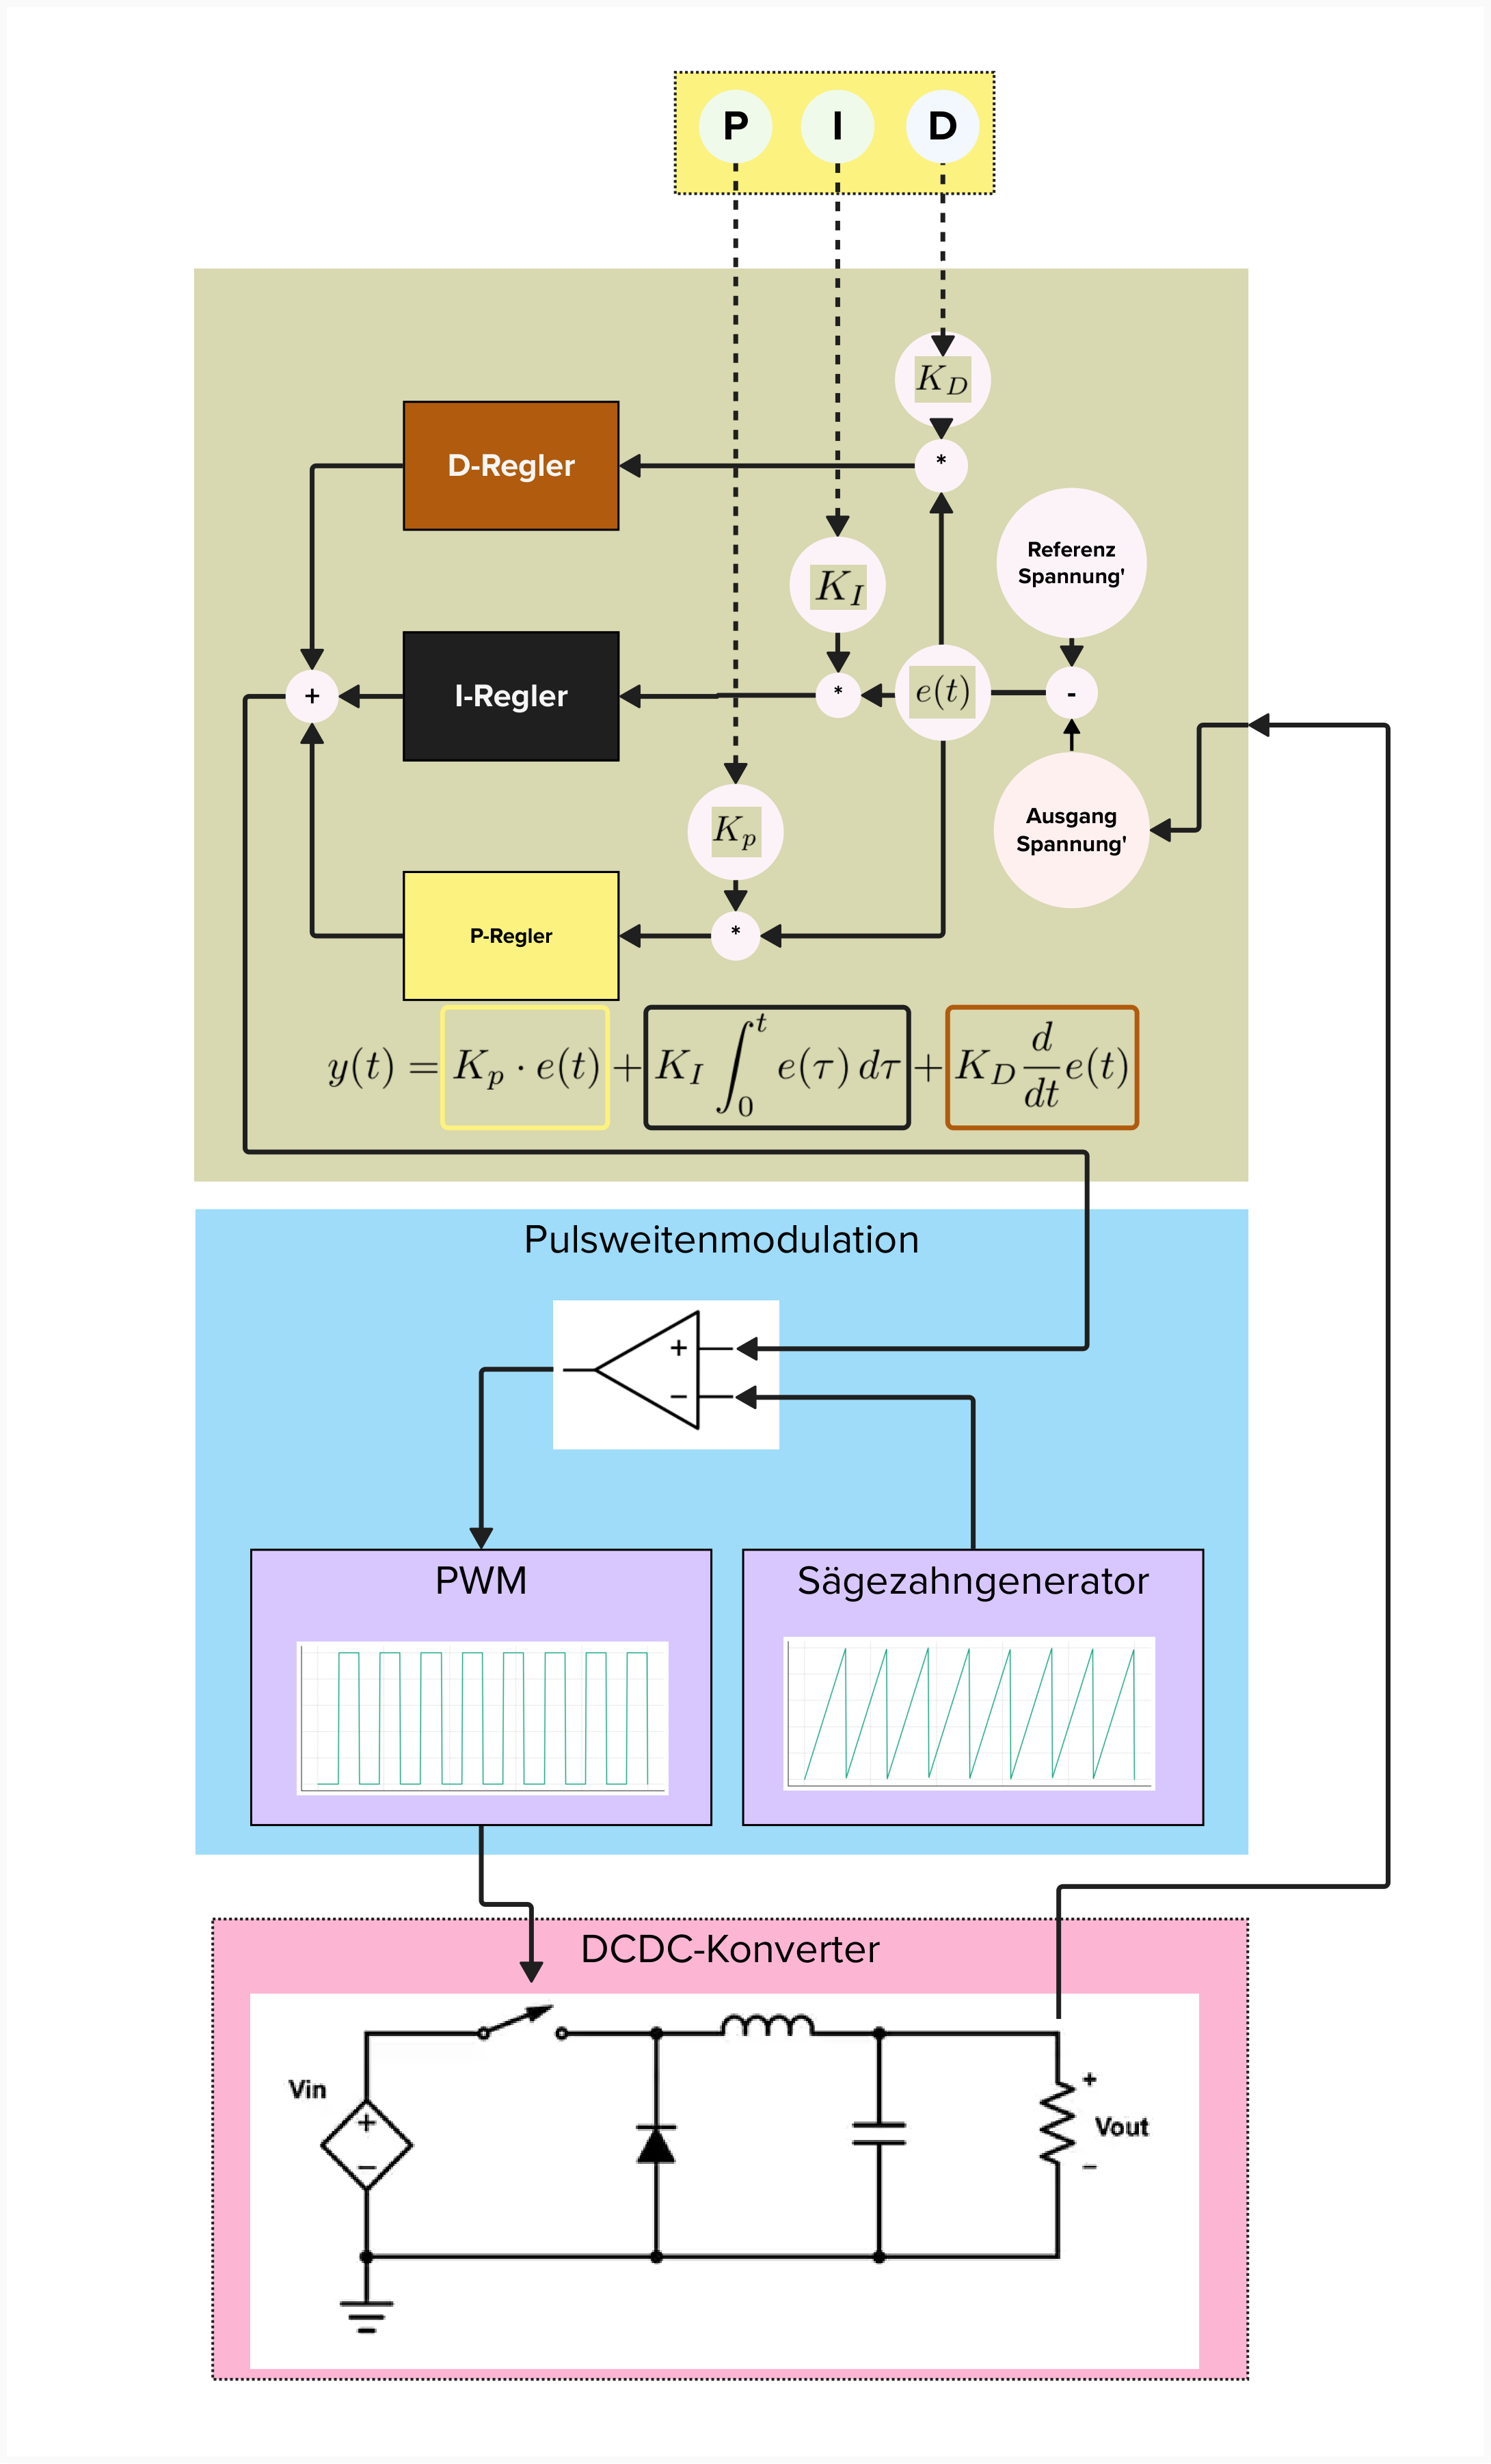
\includegraphics[width=0.99\linewidth]{3Experiment/2Experiment/3PID_Gesteuerter_DCDC_Converter.png}
    \caption{Überblick über den Regelkreis mit dem PID-Regler, PWM und DCDC-Konverter.}
    \label{fig:Regelkreis_Überblick}
\end{figure}

\subsection{Selbsttestmodul im Lernprozess des Agenten}
\label{sec:Selbsttestmodul}

Das Selbsttestmodul ist ein essentielles Element unserer Systemarchitektur, welches die Schnittstelle zwischen Theorie und Praxis repräsentiert. Es bewertet und optimiert die Effektivität der vom Agenten erlernten Schaltstrategien.

\paragraph{Funktion und Notwendigkeit des Selbsttests}
Der Selbsttest bewertet die Schaltungsreaktionen auf definierte Testszenarien, um die Lernergebnisse des Agenten zu überprüfen, wie in Abbildung \ref{fig:RewardOverTime} dargestellt.
\begin{figure}[htbp]
    \centering
    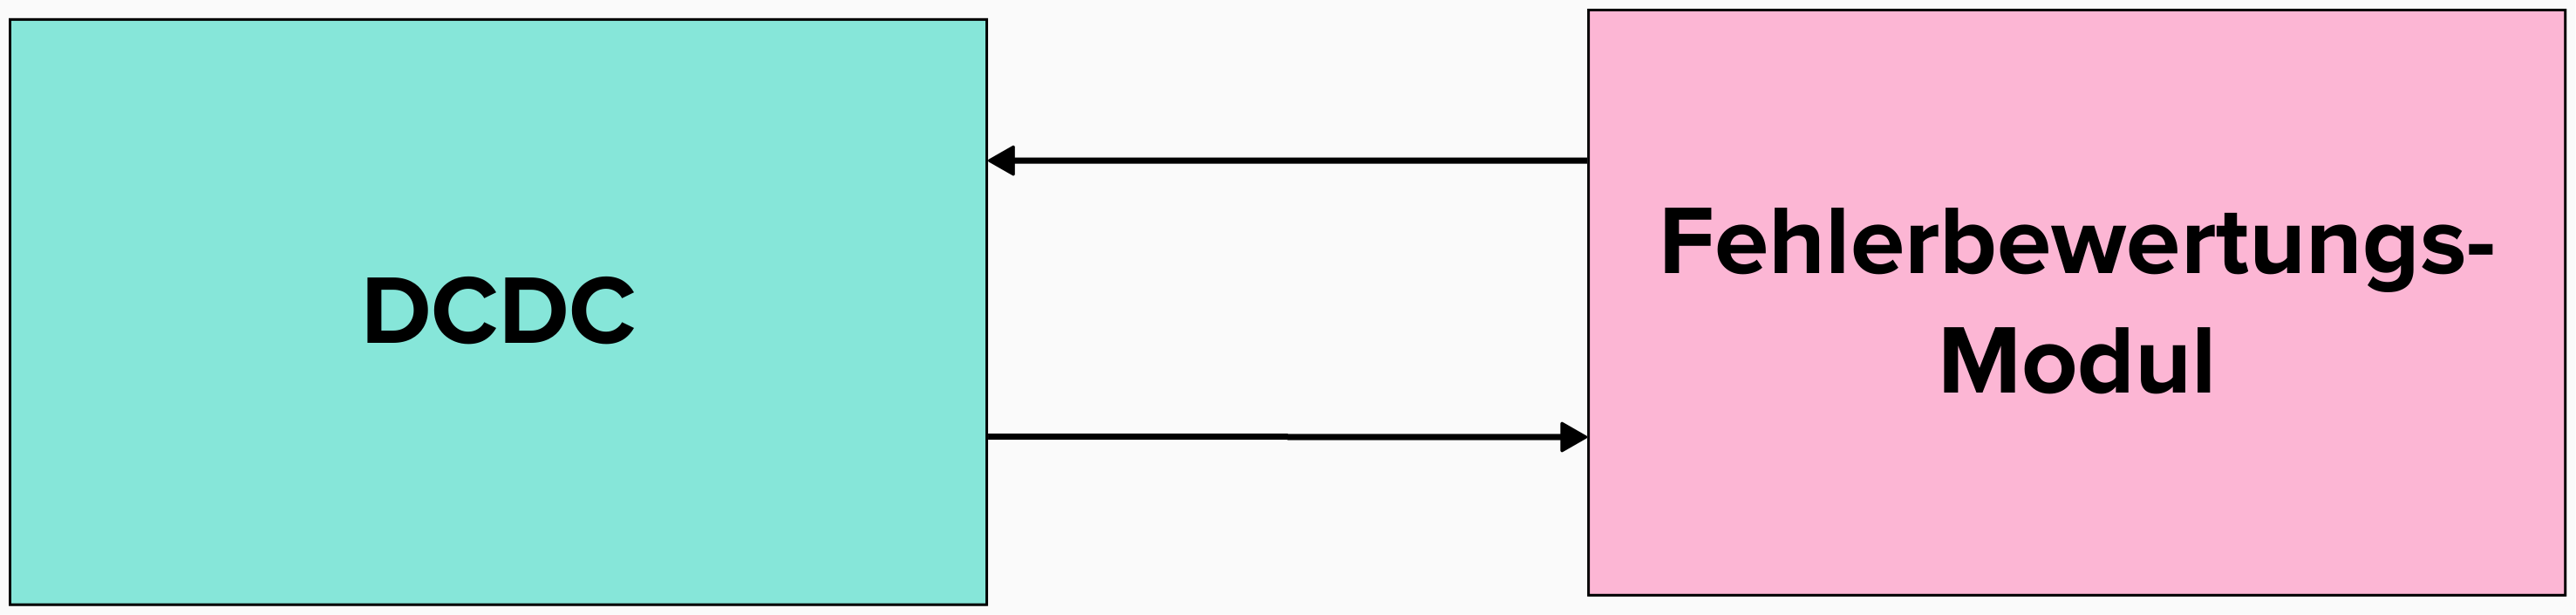
\includegraphics[width=0.5\linewidth]{3Experiment/2Experiment/4reward.png}
    \caption{Darstellung des Selbsttestmoduls im Regelkreis mit PID-Regler, PWM und DCDC-Konverter.}
    \label{fig:ControlLoop}
\end{figure}

\paragraph{Methodik der Performanzbewertung}
Die Bewertungsmethodik integriert die Abweichungen zwischen Soll- und Ist-Spannung, wobei größere Fehler durch Quadrierung stärker gewichtet werden. Extreme Spannungsspitzen werden, wie in Abbildung \ref{fig:CumulativeReward} gezeigt, exponentiell bestraft.
\begin{figure}[htbp]
    \centering
    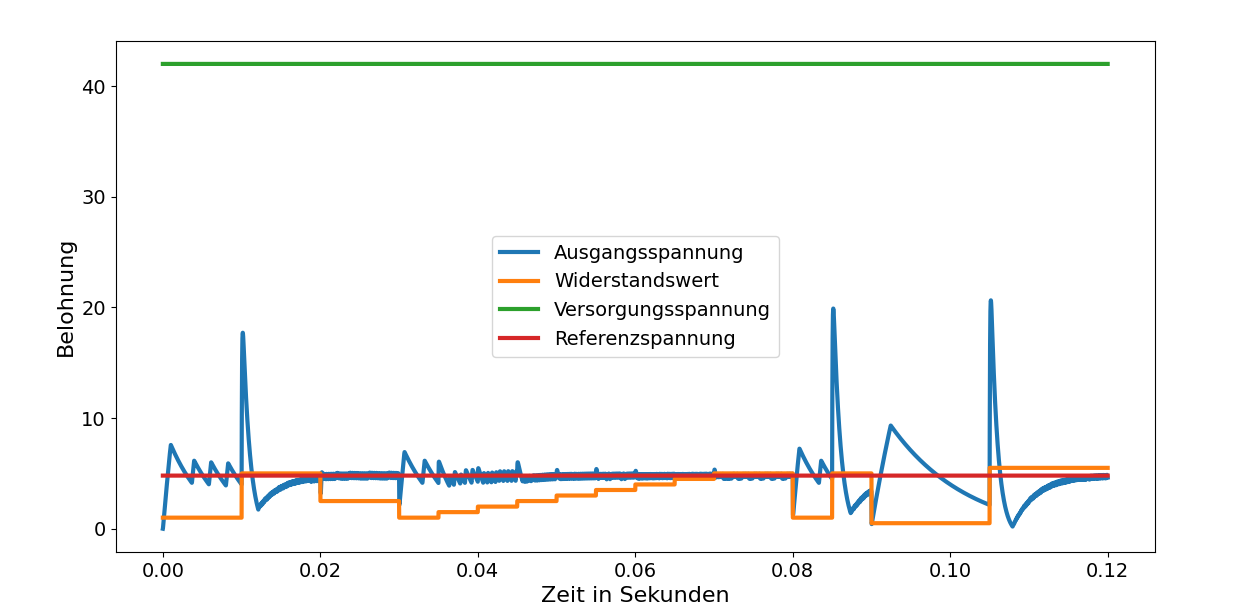
\includegraphics[width=0.99\linewidth]{3Experiment/2Experiment/4Reard_over_time.png.png}
    \caption{Visualisierung des Rewards über die Zeit während der Simulation.}
    \label{fig:RewardOverTime}
\end{figure}
\begin{figure}[htbp]
    \centering
    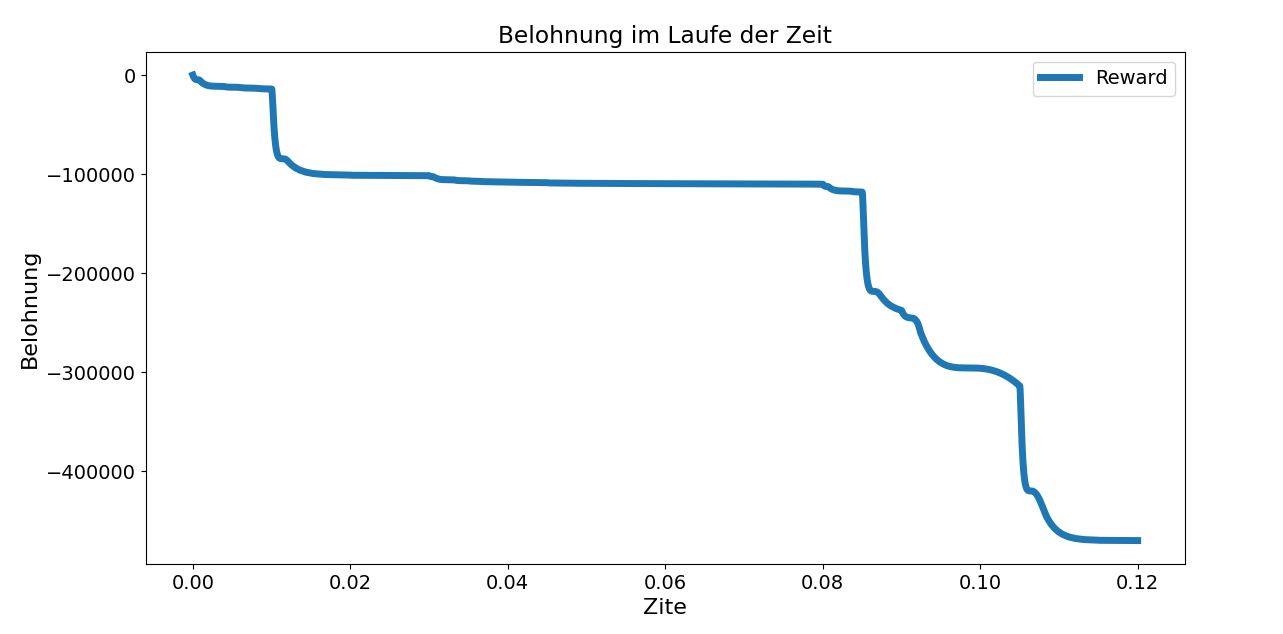
\includegraphics[width=0.99\linewidth]{3Experiment/2Experiment/4Cumulativer_Reward_Uber_Zeit.png.png}
    \caption{Kumulativer Reward über die Zeit, aufgezeichnet während der Systemtests.}
    \label{fig:CumulativeReward}
\end{figure}

\paragraph{Auswirkungen auf das Trainingsziel}
Diese Bewertungsmethodik führt zu einem quantifizierbaren Wert, der die Qualität der Regelung anzeigt und den Agenten anleitet, den Fehlerwert zu minimieren. Dies wird durch den negativen Reward widergespiegelt, der in den Lernprozess des Agenten einfließt.

\paragraph{Zeitliche Dimension der Analyse}
Selbsttests werden in wiederkehrenden Zyklen durchgeführt und bewertet, wobei der kumulierte Fehlerwert im Replay Buffer gespeichert wird, um die Strategie zu optimieren, wie in Abbildung \ref{fig:makrozyklus} illustriert.


\section{Zusammenführung des Actor-Critic-Verfahrens}
\label{sec:Synthesis_Actor_Critic}

Im vorherigen Kapitel haben wir eine Trainingsumgebung für verstärkendes Lernen etabliert, die das Sammeln von Zuständen, Aktionen und Belohnungen (Rewards) umfasst. Diese Daten werden in einem Replay Buffer gespeichert, aus dem sie entsprechend der Batch-Größe  für das Training entnommen werden.(siehe Abschnitt \ref{sec: Batch})

\paragraph{Die Dynamik des Replay Buffers}
Aus dem Replay Buffer (siehe Abschnitt  \ref{sec:Replay Buffers}) werden Datensätze extrahiert, die simultan zur Berechnung des Gradienten und zur Aktualisierung der Actor-Critic Architektur herangezogen werden.
Der Replay Buffer ist das Herzstück unserer Trainingsdynamik. Er speichert die Erfahrungen, die der Algorithmus im Laufe der Simulation macht, und ermöglicht es uns, die komplexen Zusammenhänge zwischen Aktionen und resultierenden Belohnungen zu extrahieren.

\paragraph{Die Aufgabe des Critics}
Der Critic bewertet die vom Actor ausgeführte Policy und den gegebenen Zustand,evaluiert die Effektivität der vom Actor vorgeschlagenen Aktionen im Kontext der Schaltung ( siehe Abschnitt \ref{eq:critick update}). Die generierten Schätzwerte des Critics werden mit den tatsächlichen Belohnungen verglichen, womit der Critic das Verhalten der Schaltung in Abhängigkeit von der jeweiligen Konfiguration prognostiziert. Der Critic  Durch das Abgleichen seiner Vorhersagen mit den tatsächlichen Belohnungen lernt der Critic, das Verhalten der Schaltung präzise vorherzusagen und unterstützt damit die zielgerichtete Anpassung der PID-Koeffizienten.

\paragraph{Optimierungsmechanismus des Actors}
Die Feinjustierung des Actors ist ein zentraler Bestandteil des Lernprozesses innerhalb der Actor-Critic Architektur. Anstatt komplexe Bewertungen vorzunehmen, wird ein Gradient berechnet, der die Gewichte des Actors so anpasst, dass die Schätzung des Critics in die richtige Richtung gelenkt wird, um den Reward zu maximieren (siehe Abschnitt \ref{eq:actor update}). Dieser Ansatz ermöglicht es dem Actor, aus den Prognosen des Critics zu lernen und seine Policy systematisch so zu verfeinern, dass die Belohnungsausschüttung erhöht wird. Es handelt sich hierbei um den Kern des Lernvorgangs, bei dem der Actor durch die Adjustierung seiner Gewichte basierend auf der Kritik und den Belohnungen iterativ verbessert wird.

\begin{figure}[htbp]
    \centering
		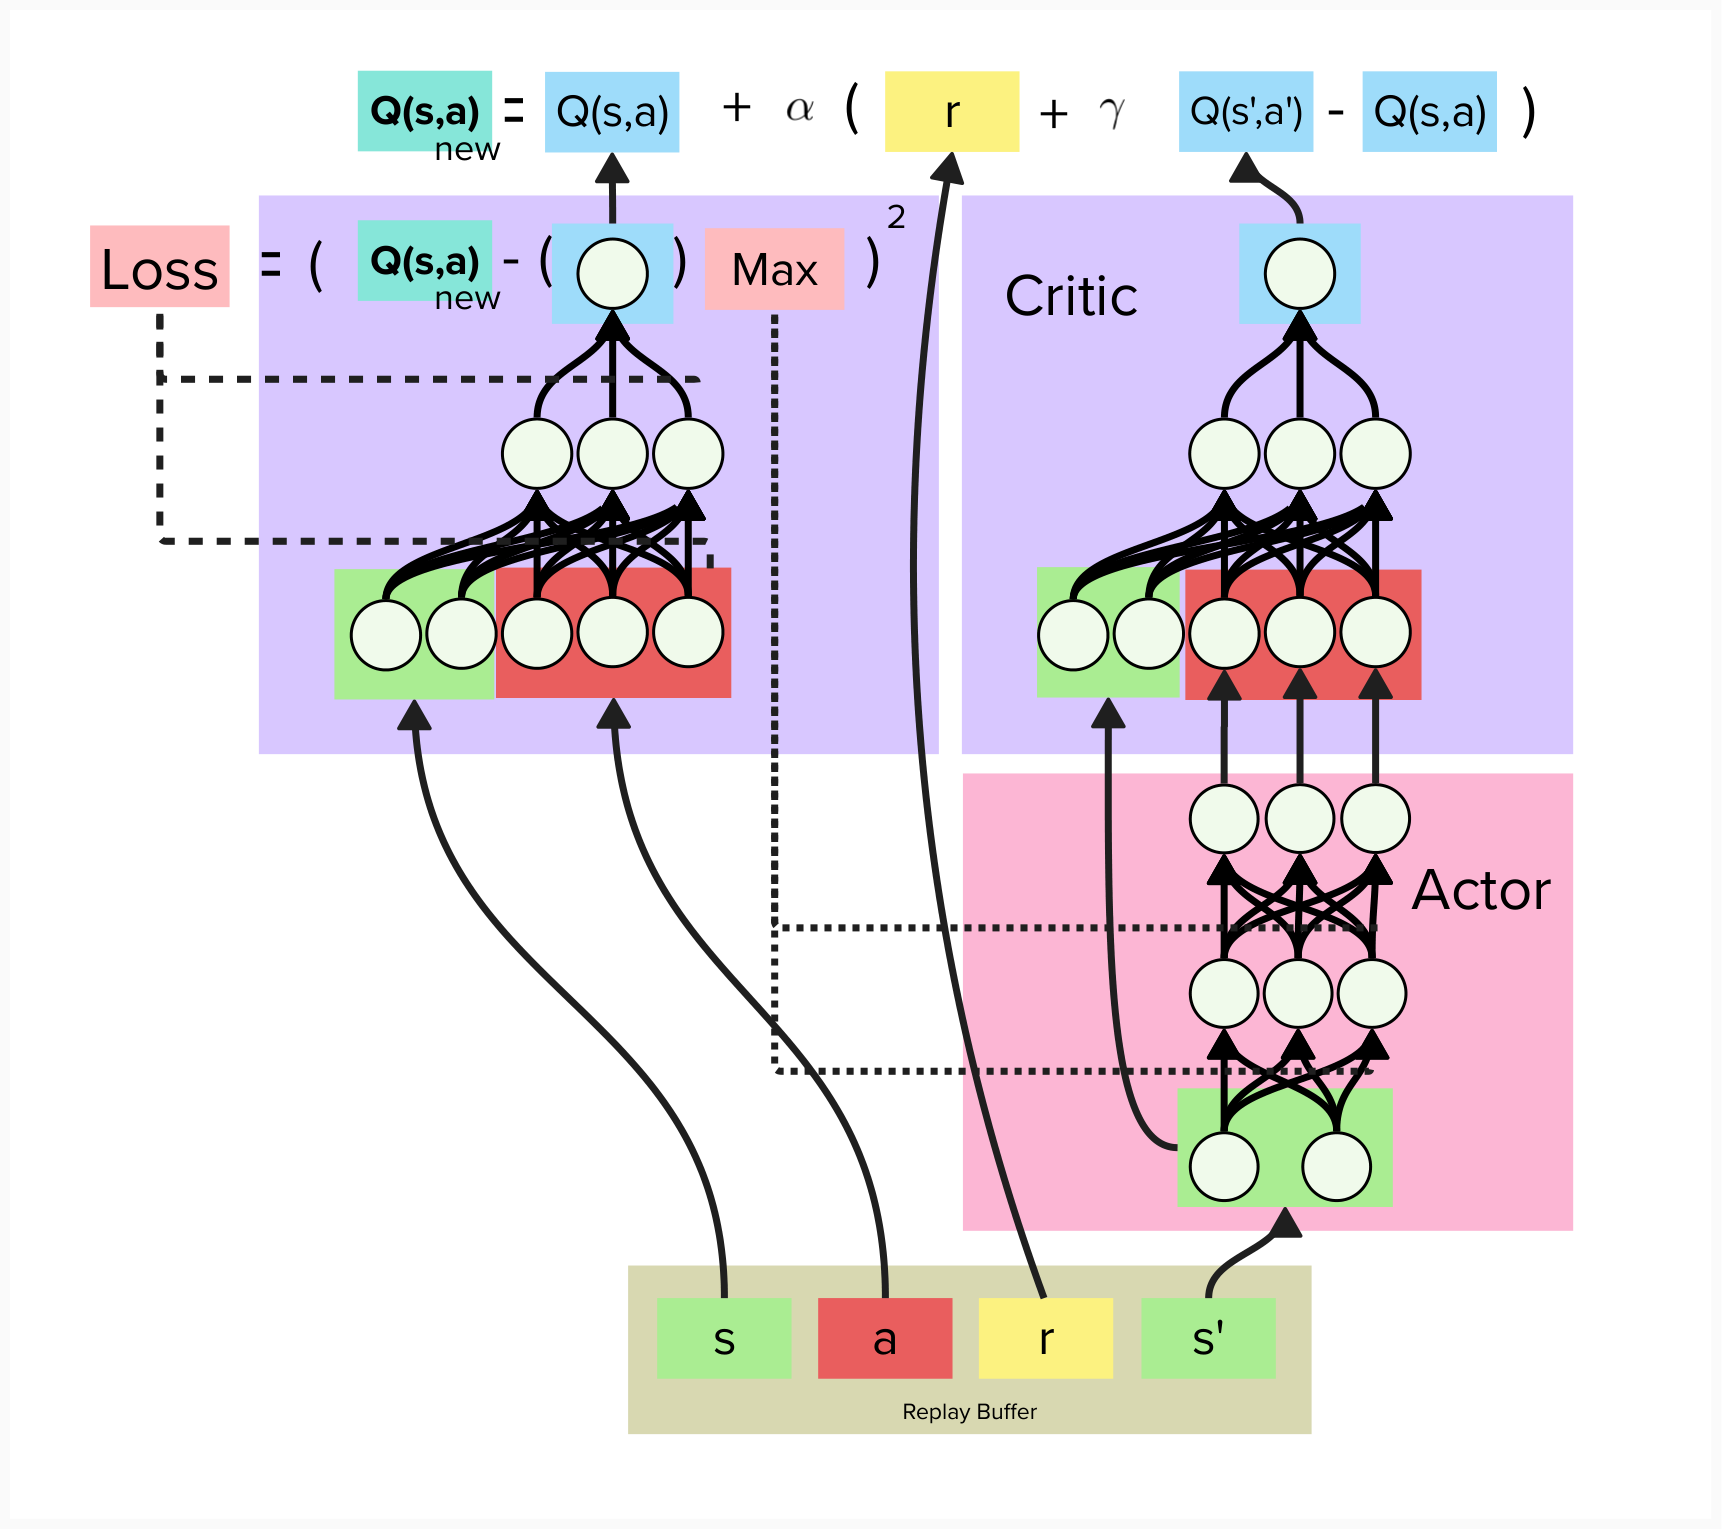
\includegraphics[width=\linewidth, trim=10px 10px 10px 10px, clip]{3Experiment/2Experiment/5Actor_Critick.png}
    \caption{Zusammengefasste Visualisierung des Update-Prozesses in der Actor-Critic Architektur.}
    \label{fig:ActorCriticSynthesis}
\end{figure}


\paragraph{Kontinuierliche Verbesserung durch Training}
Die stetige Aktualisierung des Gradienten nach jedem Simulationsschritt sorgt für eine kontinuierliche Anpassung und Verfeinerung der Actor-Critic Architektur (siehe Abschnitt \ref{sec:Synthesis_Actor_Critic}), was die Belohnungen im Laufe der Zeit maximiert. Angenommen, das Ziel ist eine direkte Optimierung der Belohnungen in unserer Simulation – die Herausforderung besteht darin, dass die komplexe Pipeline von Aktionen bis hin zum endgültigen Reward nicht mit einfachen mathematischen Mitteln abgebildet werden kann. Daher nutzen wir den Actor-Critic Ansatz, um einen einfacheren Gradienten in Bezug auf den erwarteten Reward zu maximieren, was indirekt die Optimierung der Aktionen ermöglicht.


 


% \subsection{Aufbau des Replay Buffers und Sammlung von Trainingsdaten}

Ein kritischer Schritt im Trainingsprozess des neuronalen Netzes ist die Befüllung des Replay Buffers \ref{sec:Replay Buffers}. Der Replay Buffer ist ein Speichermechanismus, der die Interaktionen des Agenten mit der Umgebung festhält, um daraus zu lernen. Er speichert Tupel \( (s, a, r, s') \), bestehend aus dem aktuellen Zustand \( s \), der vom Actor gewählten Aktion \( a \), der daraus resultierenden Belohnung \( r \) und dem nachfolgenden Zustand \( s' \).

\begin{figure}[htbp]
\centering
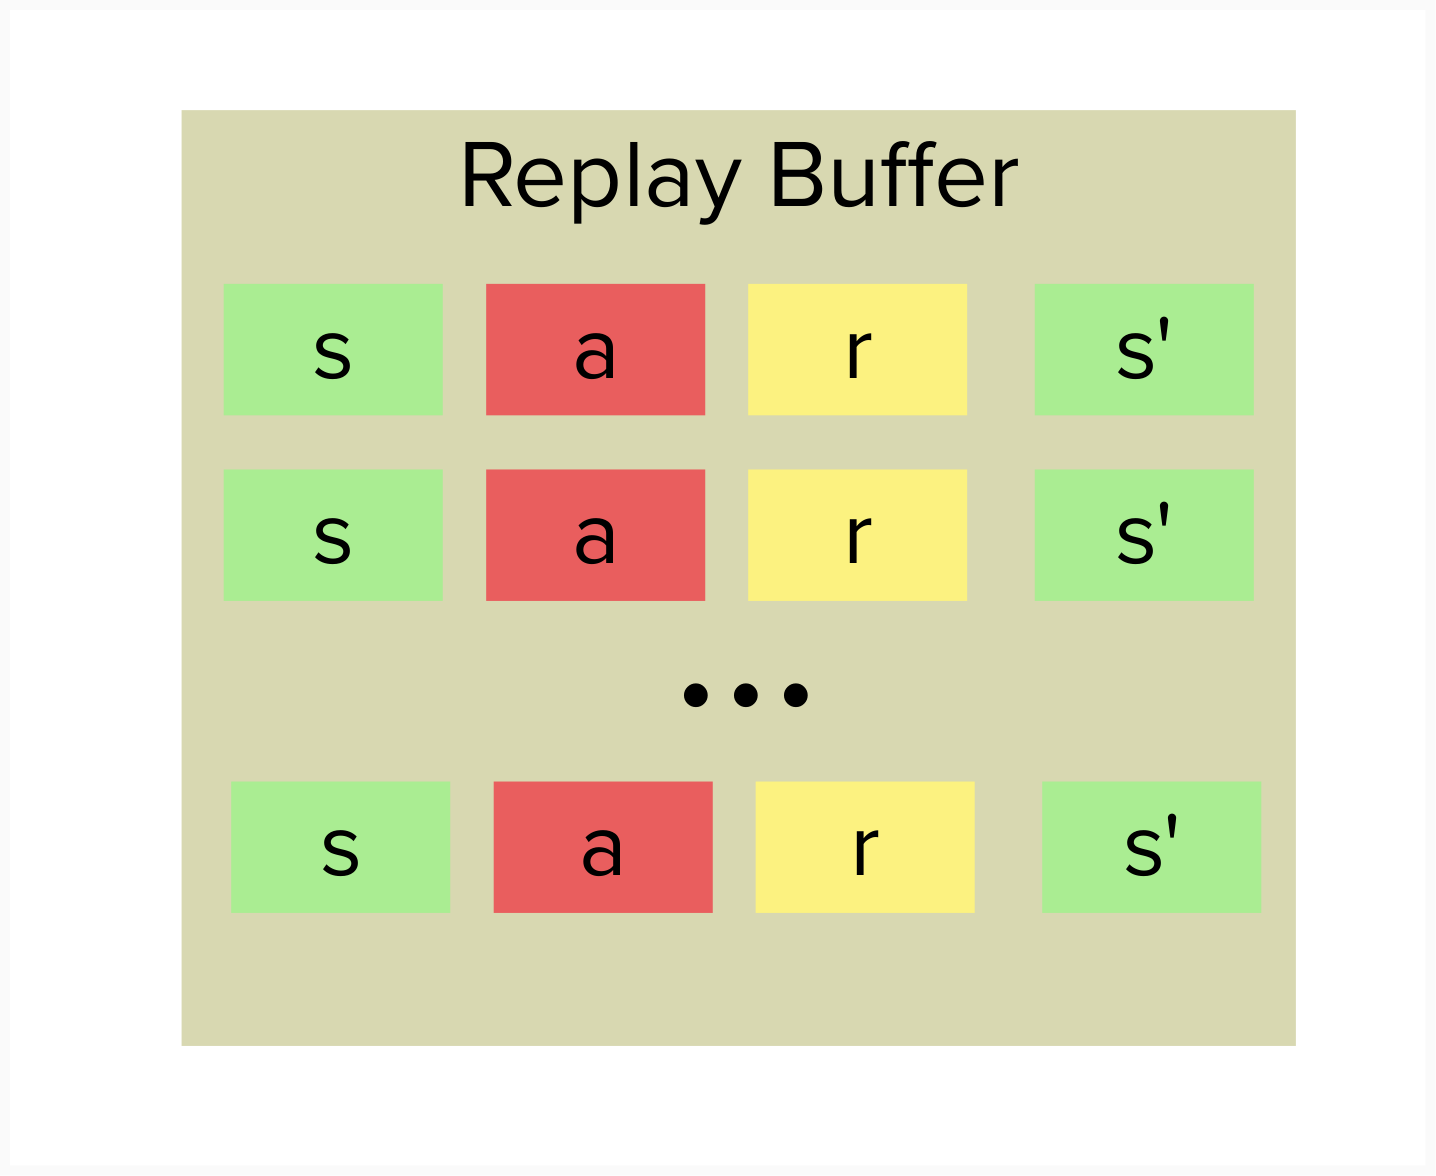
\includegraphics[width=0.5\textwidth]{3Experiment/2Experiment/1Replay_Buffer.png}
\caption{Schematische Darstellung des Replay Buffers, der die Elemente \( s \), \( a \), \( r \), und \( s' \) speichert, welche die Zustände, Aktionen, Belohnungen und Folgezustände repräsentieren.}
\label{fig:replay-buffer}
\end{figure}

Die im Replay Buffer \ref{fig:replay-buffer} gespeicherten Daten werden für das Training des neuronalen Netzes verwendet.







